\section{问题二：固定轮廓互连线长模型的建立与求解}

为了在给定死区率的正方形轮廓内降低模块互连线长，本问沿“网络驱动目标位置—几何合法化—局部线长优化”的技术主线展开：先由网络连接与固定 Terminal 提取模块的目标中心，再将这些连续目标转化为满足固定边界和非重叠约束的离散布局，最后修正合法化造成的局部线长损失。

\subsection{固定轮廓与 HPWL 优化模型}

\subsubsection{连续轮廓与整数坐标边界}

设硬模块总面积为 $A_{\mathrm{block}}$，题目给定死区率 $\Gamma=0.15$。按死区率定义，正方形轮廓面积及连续边长为
\begin{equation}
  A_{\mathrm{outline}}=(1+\Gamma)A_{\mathrm{block}},
  \qquad
  L_{\mathrm{box}}=\sqrt{(1+\Gamma)A_{\mathrm{block}}}.
  \label{eq:q2_outline}
\end{equation}
模块尺寸和模块坐标均为整数，因此模块右边界和上边界也是整数。令
\begin{equation}
  G=\lfloor L_{\mathrm{box}}\rfloor,
  \label{eq:q2_grid_side}
\end{equation}
则整数坐标下的 $x_i+w_i\le L_{\mathrm{box}}$ 与 $x_i+w_i\le G$ 等价，纵向边界同理。$G$ 仅用于确定整数坐标，轮廓面积仍由连续边长 $L_{\mathrm{box}}$ 按式~\eqref{eq:q2_outline}计算。由三组模块总面积得到的固定轮廓参数见表~\ref{tab:q2_outline_parameters}。

\begin{table}[H]
  \centering
  \caption{问题二固定正方形轮廓参数}
  \label{tab:q2_outline_parameters}
  \small
  \begin{tabular}{lrrrr}
    \toprule
    实例 & $A_{\mathrm{block}}$ & $L_{\mathrm{box}}$ & $G$ & $A_{\mathrm{outline}}$ \\
    \midrule
    \texttt{n100} & 179501 & 454.341 & 454 & 206426.150 \\
    \texttt{n200} & 175696 & 449.500 & 449 & 202050.400 \\
    \texttt{n300} & 273170 & 560.487 & 560 & 314145.500 \\
    \bottomrule
  \end{tabular}
\end{table}

由此先得到连续轮廓边长 $L_{\mathrm{box}}$，再由 $G$ 刻画与整数模块坐标等价的边界。问题二沿用问题一的旋转变量 $r_i$ 和旋转后尺寸 $(w_i,h_i)$；在固定正方形轮廓内，每个模块必须满足
\begin{equation}
  0\le x_i,\quad 0\le y_i,\quad
  x_i+w_i\le L_{\mathrm{box}},\quad y_i+h_i\le L_{\mathrm{box}}.
  \label{eq:q2_boundary}
\end{equation}
任意两个模块仍满足式~\eqref{eq:q1_nonoverlap}的方向分离约束。式~\eqref{eq:q2_boundary}与非重叠约束共同定义本问的几何可行域。

\subsubsection{模块中心、HPWL 与优化目标}

在上述整数坐标可行域中，模块引脚位于几何中心，因此模块 $i$ 的引脚坐标为
\begin{equation}
  \boldsymbol{c}_i=\left(x_i+\frac{w_i}{2},\ y_i+\frac{h_i}{2}\right).
  \label{eq:q2_block_center}
\end{equation}
若引脚 $p$ 属于硬模块，则 $(X_p,Y_p)=\boldsymbol{c}_i$；若其为外部终端，则 $(X_p,Y_p)$ 取 \texttt{.pl} 中的固定坐标。对网络 $e$，其半周长线长为
\begin{equation}
  \ell_e=
  \left(\max_{p\in\mathcal{P}_e}X_p-\min_{p\in\mathcal{P}_e}X_p\right)
  +
  \left(\max_{p\in\mathcal{P}_e}Y_p-\min_{p\in\mathcal{P}_e}Y_p\right).
  \label{eq:q2_net_hpwl}
\end{equation}
该指标等于网络所有引脚最小轴对齐外接矩形的半周长。全部网络的总 HPWL 为
\begin{equation}
  \mathcal{L}=\sum_{e\in\mathcal{E}}\ell_e.
  \label{eq:q2_total_hpwl}
\end{equation}

第二问要求在固定轮廓可行域内最小化式~\eqref{eq:q2_total_hpwl}，可写为
\begin{equation}
  \begin{aligned}
    \min_{\{x_i,y_i,r_i\}}\quad & \mathcal{L},\\
    \text{s.t.}\quad
      & r_i\in\{0,1\},\quad x_i,y_i\in\mathbb{Z}_{\ge0},\\
      & \text{式~\eqref{eq:q1_rotation}、\eqref{eq:q1_nonoverlap}和~\eqref{eq:q2_boundary}}.
  \end{aligned}
  \label{eq:q2_model}
\end{equation}
至此，连续边长 $L_{\mathrm{box}}$ 决定物理轮廓，整数边界 $G$ 决定坐标可行域，模块中心将几何位置映射为网络引脚位置，单网 HPWL 再汇总为总 HPWL，最终形成式~\eqref{eq:q2_model}的优化目标。由于旋转、坐标和模块相对位置均为离散决策，且非重叠条件为析取约束，下面采用分层方法在网络方向与几何可行性之间建立联系。

\subsection{求解方法：网络驱动合法化与局部重插入}

\subsubsection{二次线长松弛}

为获得模块在网络连接意义下的空间方向，暂时忽略非重叠约束，并以二次线长近似代替分段线性的 HPWL~\cite{eisenmann1998}。对引脚数为 $d_e$ 的网络，将其引脚两两连接成团，权重取 $1/(d_e-1)$，求解
\begin{equation}
  \min_{\{\boldsymbol{z}_i\}}
  \sum_{e\in\mathcal{E}}\frac{1}{d_e-1}
  \sum_{\substack{u<v\\u,v\in\mathcal{P}_e}}
  \lVert\boldsymbol{z}_u-\boldsymbol{z}_v\rVert_2^2,
  \label{eq:q2_quadratic_relaxation}
\end{equation}
其中外部 Terminal 位置保持固定，硬模块中心为待求变量。式~\eqref{eq:q2_quadratic_relaxation}形成图拉普拉斯线性方程，求解后将模块中心投影到轮廓坐标范围，得到目标中心 $\widehat{\boldsymbol{c}}_i$。必须强调，该松弛解只用于提供网络驱动的空间方向：它既未满足模块非重叠等离散几何约束，也不是最终 HPWL 解。

\subsubsection{目标引导几何合法化}

二次松弛得到的目标中心通常彼此重叠，不能直接作为模块坐标。合法化虽然能够消除越界与重叠，却会迫使模块偏离其网络目标位置；而逐个放置的先后关系还会改变剩余空间形态，使早期几何决策被后续模块继承。因此，合法化并非单纯的可行性修补，它可能破坏松弛解中已经形成的网络邻近结构，并成为最终 HPWL 的重要来源。

为降低这种损失，本文在固定轮廓的可用矩形区域内逐个插入模块，使候选位置同时参考目标中心、已放置相邻引脚与固定 Terminal 所提供的局部网络信息，并在两种旋转方向下检验边界和重叠约束。考虑到模块顺序会形成不同的空间分割结构，再以网络连接、模块几何特征和目标中心位置构造多种初始顺序，并以不同侧重点的插入准则扩充可行初值。最终统一按精确总 HPWL 比较这些合法布局。

\subsubsection{局部重插入：合法化损失的二次修正}

几何合法化首先保证可行，但未必使每个模块处于对其关联网络最有利的位置。为对这部分线长损失进行二次修正，本文按模块的 HPWL 贡献依次尝试单模块重插入：\texttt{n100} 在移除模块后重新确定可用矩形区域，\texttt{n200} 和 \texttt{n300} 则利用相邻引脚、Terminal 与目标中心形成的 HPWL 断点控制搜索规模。每次调整均重新检验几何约束，且只有精确总 HPWL 严格下降时才接受，从而在不破坏合法性的前提下恢复部分网络邻近关系。当前实现仅对初始 HPWL 较小的若干布局进行有限轮局部修正；具体预算为前 $3$ 个布局和 $2$ 轮迭代。

第二问的求解步骤如下：
\begin{enumerate}
  \item 读取模块、网络和终端数据，计算 $A_{\mathrm{block}}$、$L_{\mathrm{box}}$ 与 $G$；
  \item 求解二次线长松弛，得到模块目标中心；
  \item 组合多种初始顺序和插入准则，在 $G\times G$ 整数坐标区域内得到可行布局；
  \item 对较优初始布局进行局部重插入，修正合法化造成的线长损失；
  \item 根据最终模块坐标重新计算 HPWL，并选择其中最小的可行布局；
  \item 检验模块完整性、边界、重叠、面积与 HPWL 一致性，得到模块坐标和布局图。
\end{enumerate}

解析松弛需要求解规模为模块数的线性方程组，稠密实现的计算复杂度为 $O(n^3)$；合法化与局部重插入还需反复检验候选区域和模块冲突，因此大规模实例采用 HPWL 断点搜索控制计算量。

\subsection{求解结果与分析}

\subsubsection{HPWL 求解结果}

表~\ref{tab:q2_main_results}给出各实例经过局部优化后的 HPWL 最小可行布局。局部改善率以对应合法化初始布局的 HPWL 为基准计算。

\begin{table}[H]
  \centering
  \caption{问题二固定轮廓下的 HPWL 优化结果}
  \label{tab:q2_main_results}
  \small
  \resizebox{\textwidth}{!}{%
  \begin{tabular}{lrrrrrl}
    \toprule
    实例 & $L_{\mathrm{box}}$ & 初始 HPWL & 最终 HPWL & 改善率/\% & 有效移动次数 & 局部改进方法 \\
    \midrule
    \texttt{n100} & 454.341 & 224273.0 & 220279.0 & 1.7809 & 44 & 精确空矩形重插入 \\
    \texttt{n200} & 449.500 & 411599.0 & 410072.5 & 0.3709 & 20 & HPWL 断点搜索 \\
    \texttt{n300} & 560.487 & 563981.0 & 560492.5 & 0.6185 & 34 & HPWL 断点搜索 \\
    \bottomrule
  \end{tabular}%
  }
\end{table}

三组数据经过局部重插入后 HPWL 均继续下降：\texttt{n100} 由 $224273.0$ 降至 $220279.0$，改善 $1.7809\%$；\texttt{n200} 与 \texttt{n300} 分别改善 $0.3709\%$ 和 $0.6185\%$。这说明几何合法化虽然已经给出可行布局，但模块相对位置中仍保留可被局部移动利用的线长优化空间，也验证了“合法化后再修正”这一层次的必要性。为直观比较三组数据的变化，将表中优化前后的 HPWL 绘于图~\ref{fig:q2_hpwl_before_after}。

\begin{figure}[H]
  \centering
  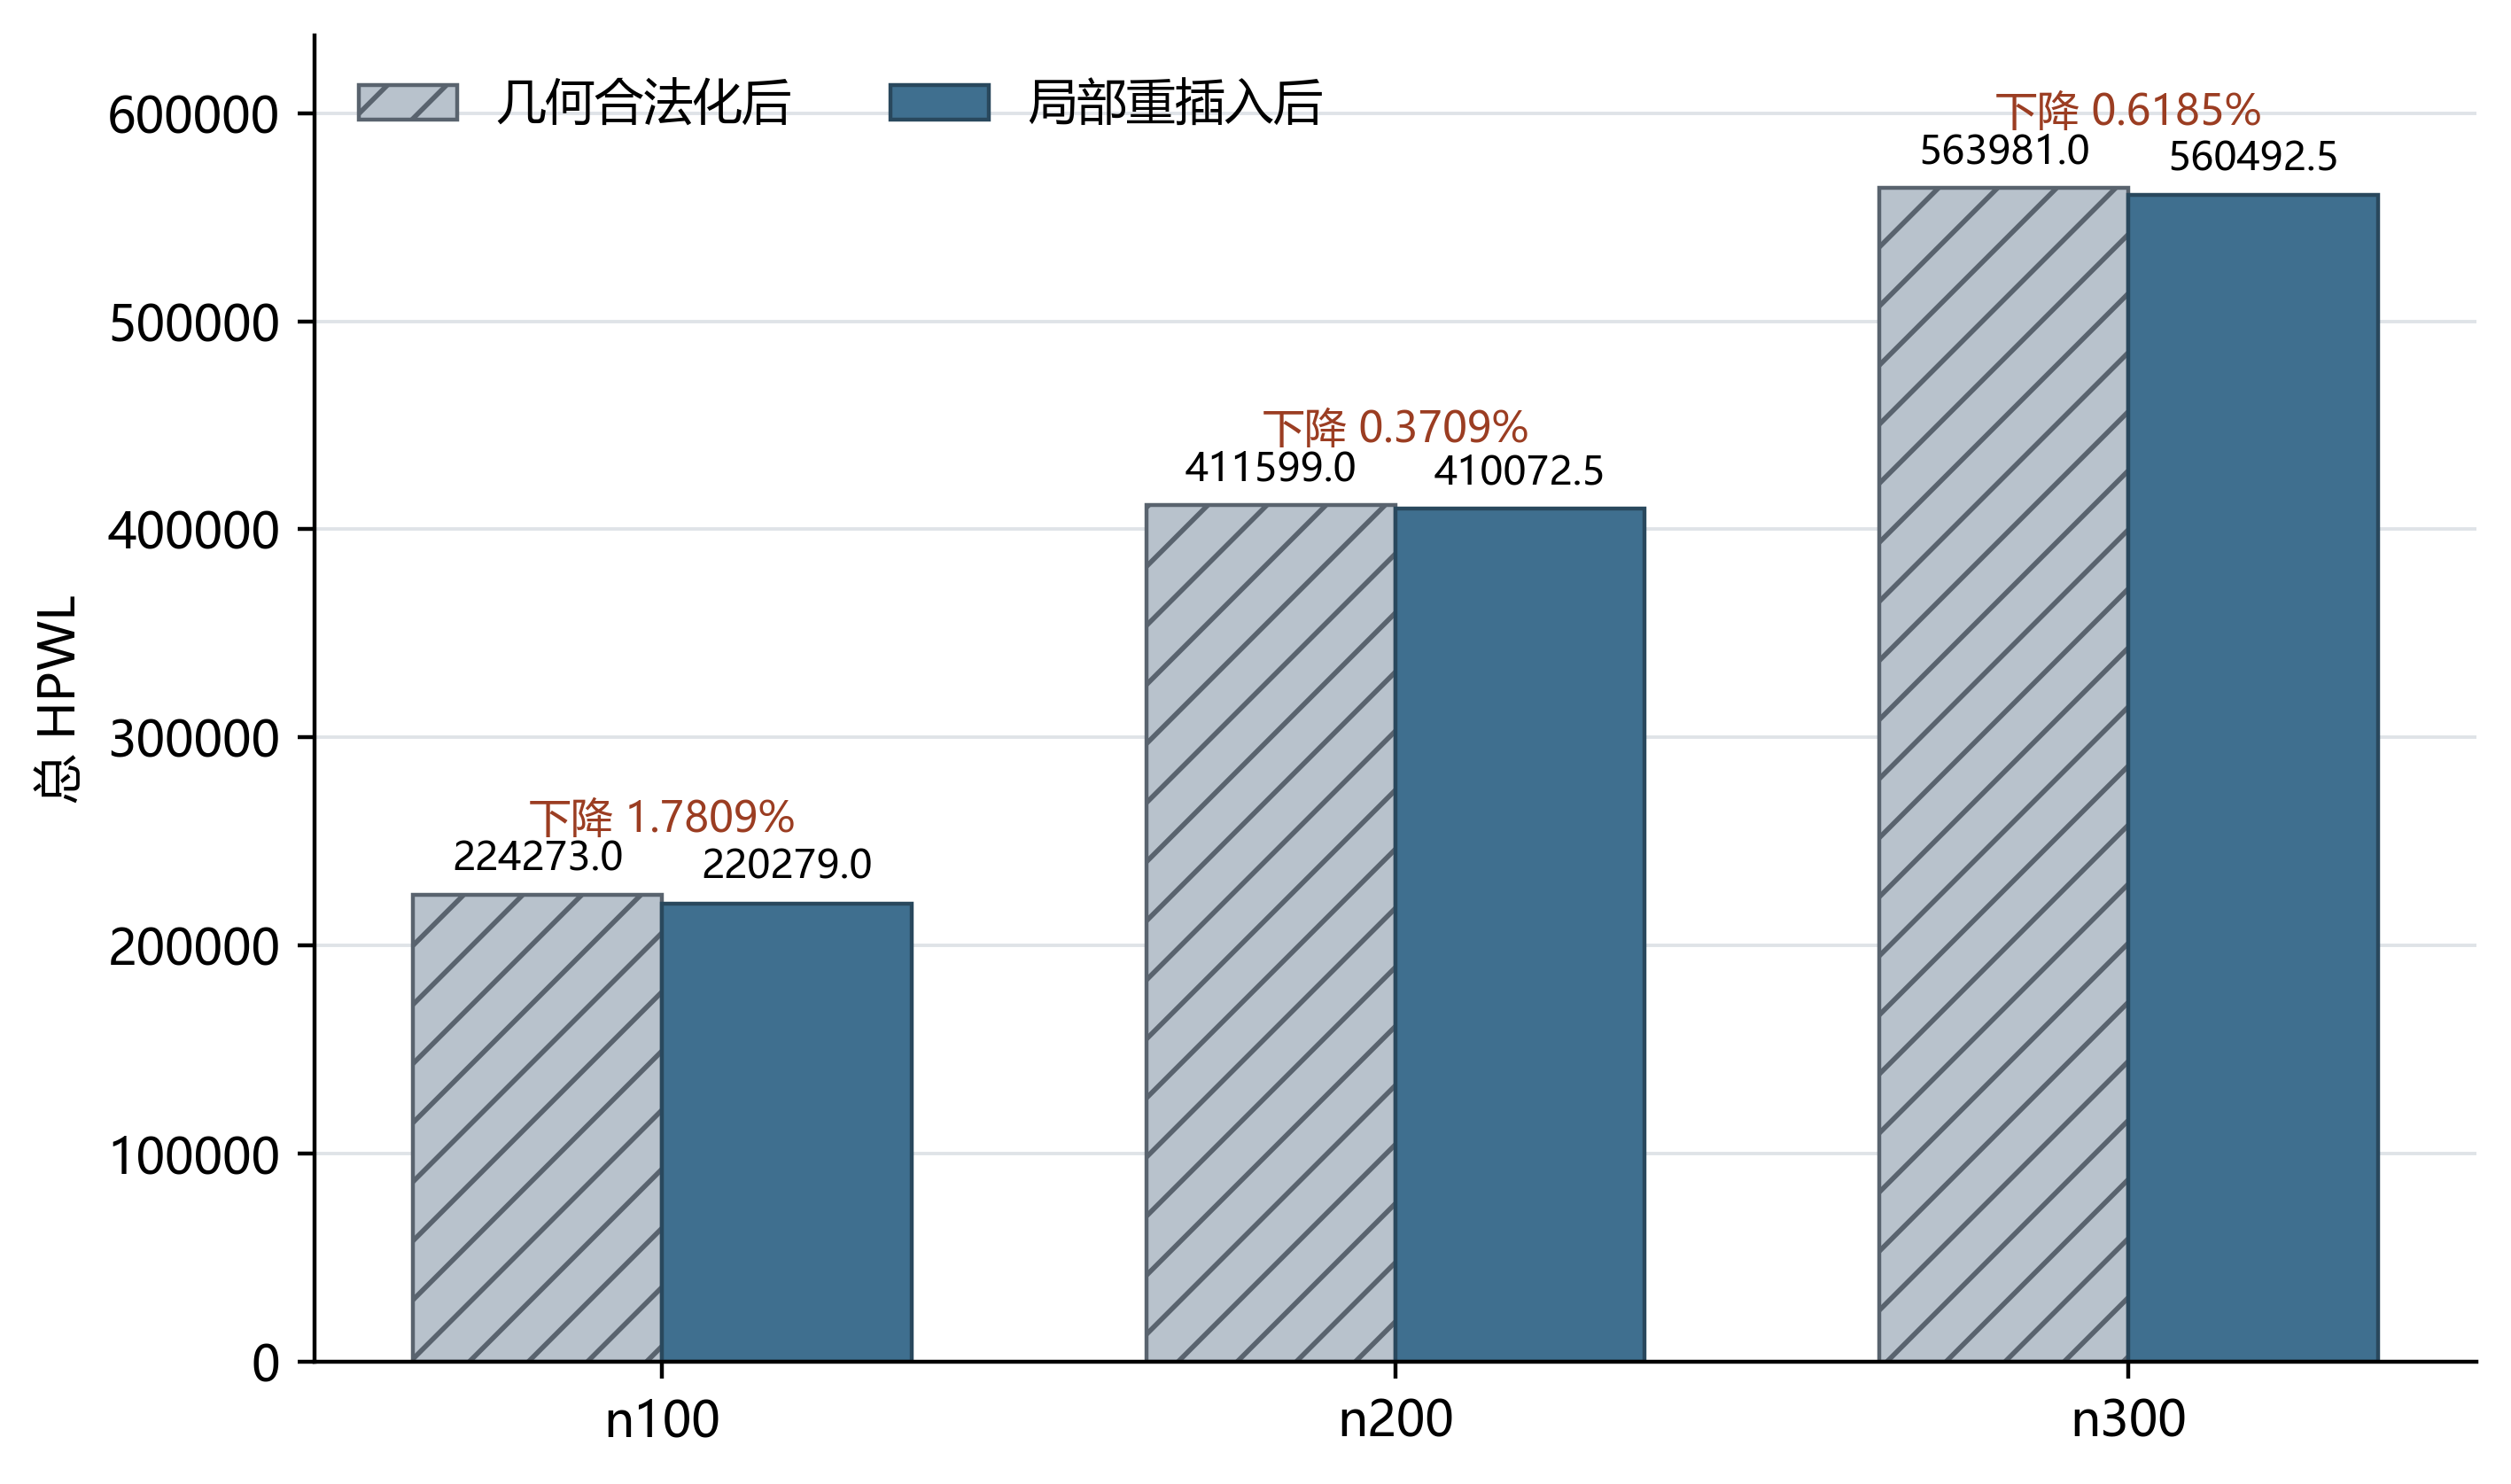
\includegraphics[width=0.78\textwidth]{../results/q2/figures/q2_hpwl_before_after.png}
  \caption{三组实例在几何合法化后与局部重插入后的 HPWL 对比}
  \label{fig:q2_hpwl_before_after}
\end{figure}

图中三组柱对均呈下降关系，其中 \texttt{n100} 的相对降幅最大；\texttt{n200} 和 \texttt{n300} 的降幅较小但方向一致。局部优化的作用因而不是重新构造布局，而是在固定轮廓和既有空间分割结构下，进一步回收合法化造成的局部线长损失。

\subsubsection{初始布局依赖性分析}

表~\ref{tab:q2_candidate_comparison}并非一般的方法优劣对照，而用于考察初始合法化结构对最终结果的影响。每组实例列出三个代表性合法布局及其局部优化结果，表内 HPWL 均由对应布局坐标按同一公式重新计算。

\begin{table}[H]
  \centering
  \caption{问题二局部搜索结果对初始合法化布局的依赖性}
  \label{tab:q2_candidate_comparison}
  \small
  \begin{tabular}{l p{4.4cm} rrr}
    \toprule
    实例 & 方法组合 & 初始 HPWL & 改进后 HPWL & 有效移动次数 \\
    \midrule
    \texttt{n100} & \texttt{degree\_area+wire} & 224273.0 & 220279.0 & 44 \\
    \texttt{n100} & \texttt{shelf\_bfd:native} & 242944.0 & 233349.0 & 109 \\
    \texttt{n100} & \texttt{area\_degree+target} & 243190.5 & 234380.5 & 32 \\
    \midrule
    \texttt{n200} & \texttt{target\_yx+wire} & 411599.0 & 410072.5 & 20 \\
    \texttt{n200} & \texttt{degree\_area+wire} & 413258.0 & 412640.5 & 27 \\
    \texttt{n200} & \texttt{area\_degree+wire} & 420230.5 & 417335.0 & 47 \\
    \midrule
    \texttt{n300} & \texttt{target\_xy+wire} & 563981.0 & 560492.5 & 34 \\
    \texttt{n300} & \texttt{target\_yx+wire} & 582961.5 & 576107.0 & 59 \\
    \texttt{n300} & \texttt{degree\_area+wire} & 600456.5 & 593534.5 & 47 \\
    \bottomrule
  \end{tabular}
\end{table}

表中所有代表性布局经过局部搜索后 HPWL 均下降，说明局部修正具有一致作用；但同一实例的改进后 HPWL 仍存在明显差异。其原因在于，不同初始顺序和插入准则会在合法化阶段形成不同的模块邻接关系与剩余空间分割，而单模块局部搜索只能在既有结构附近调整，难以跨越较大的结构性差异。因此，局部搜索不能完全消除初始合法化的影响，构造多初值并从中筛选具有必要性。这也表明，最终 HPWL 不仅取决于局部移动能力，更取决于网络驱动信息在合法化阶段被保留的程度。

为展示固定轮廓内的模块分布及线长压力，将 \texttt{n100} 和 \texttt{n200} 的布局并列绘于图~\ref{fig:q2_n100_n200}。图中低饱和色矩形表示普通硬模块，黑点表示固定 Terminal，统一强调色矩形表示 HPWL 较高网络的引脚外接框。

\begin{figure}[H]
  \centering
  \begin{minipage}[c]{0.48\textwidth}
    \centering
    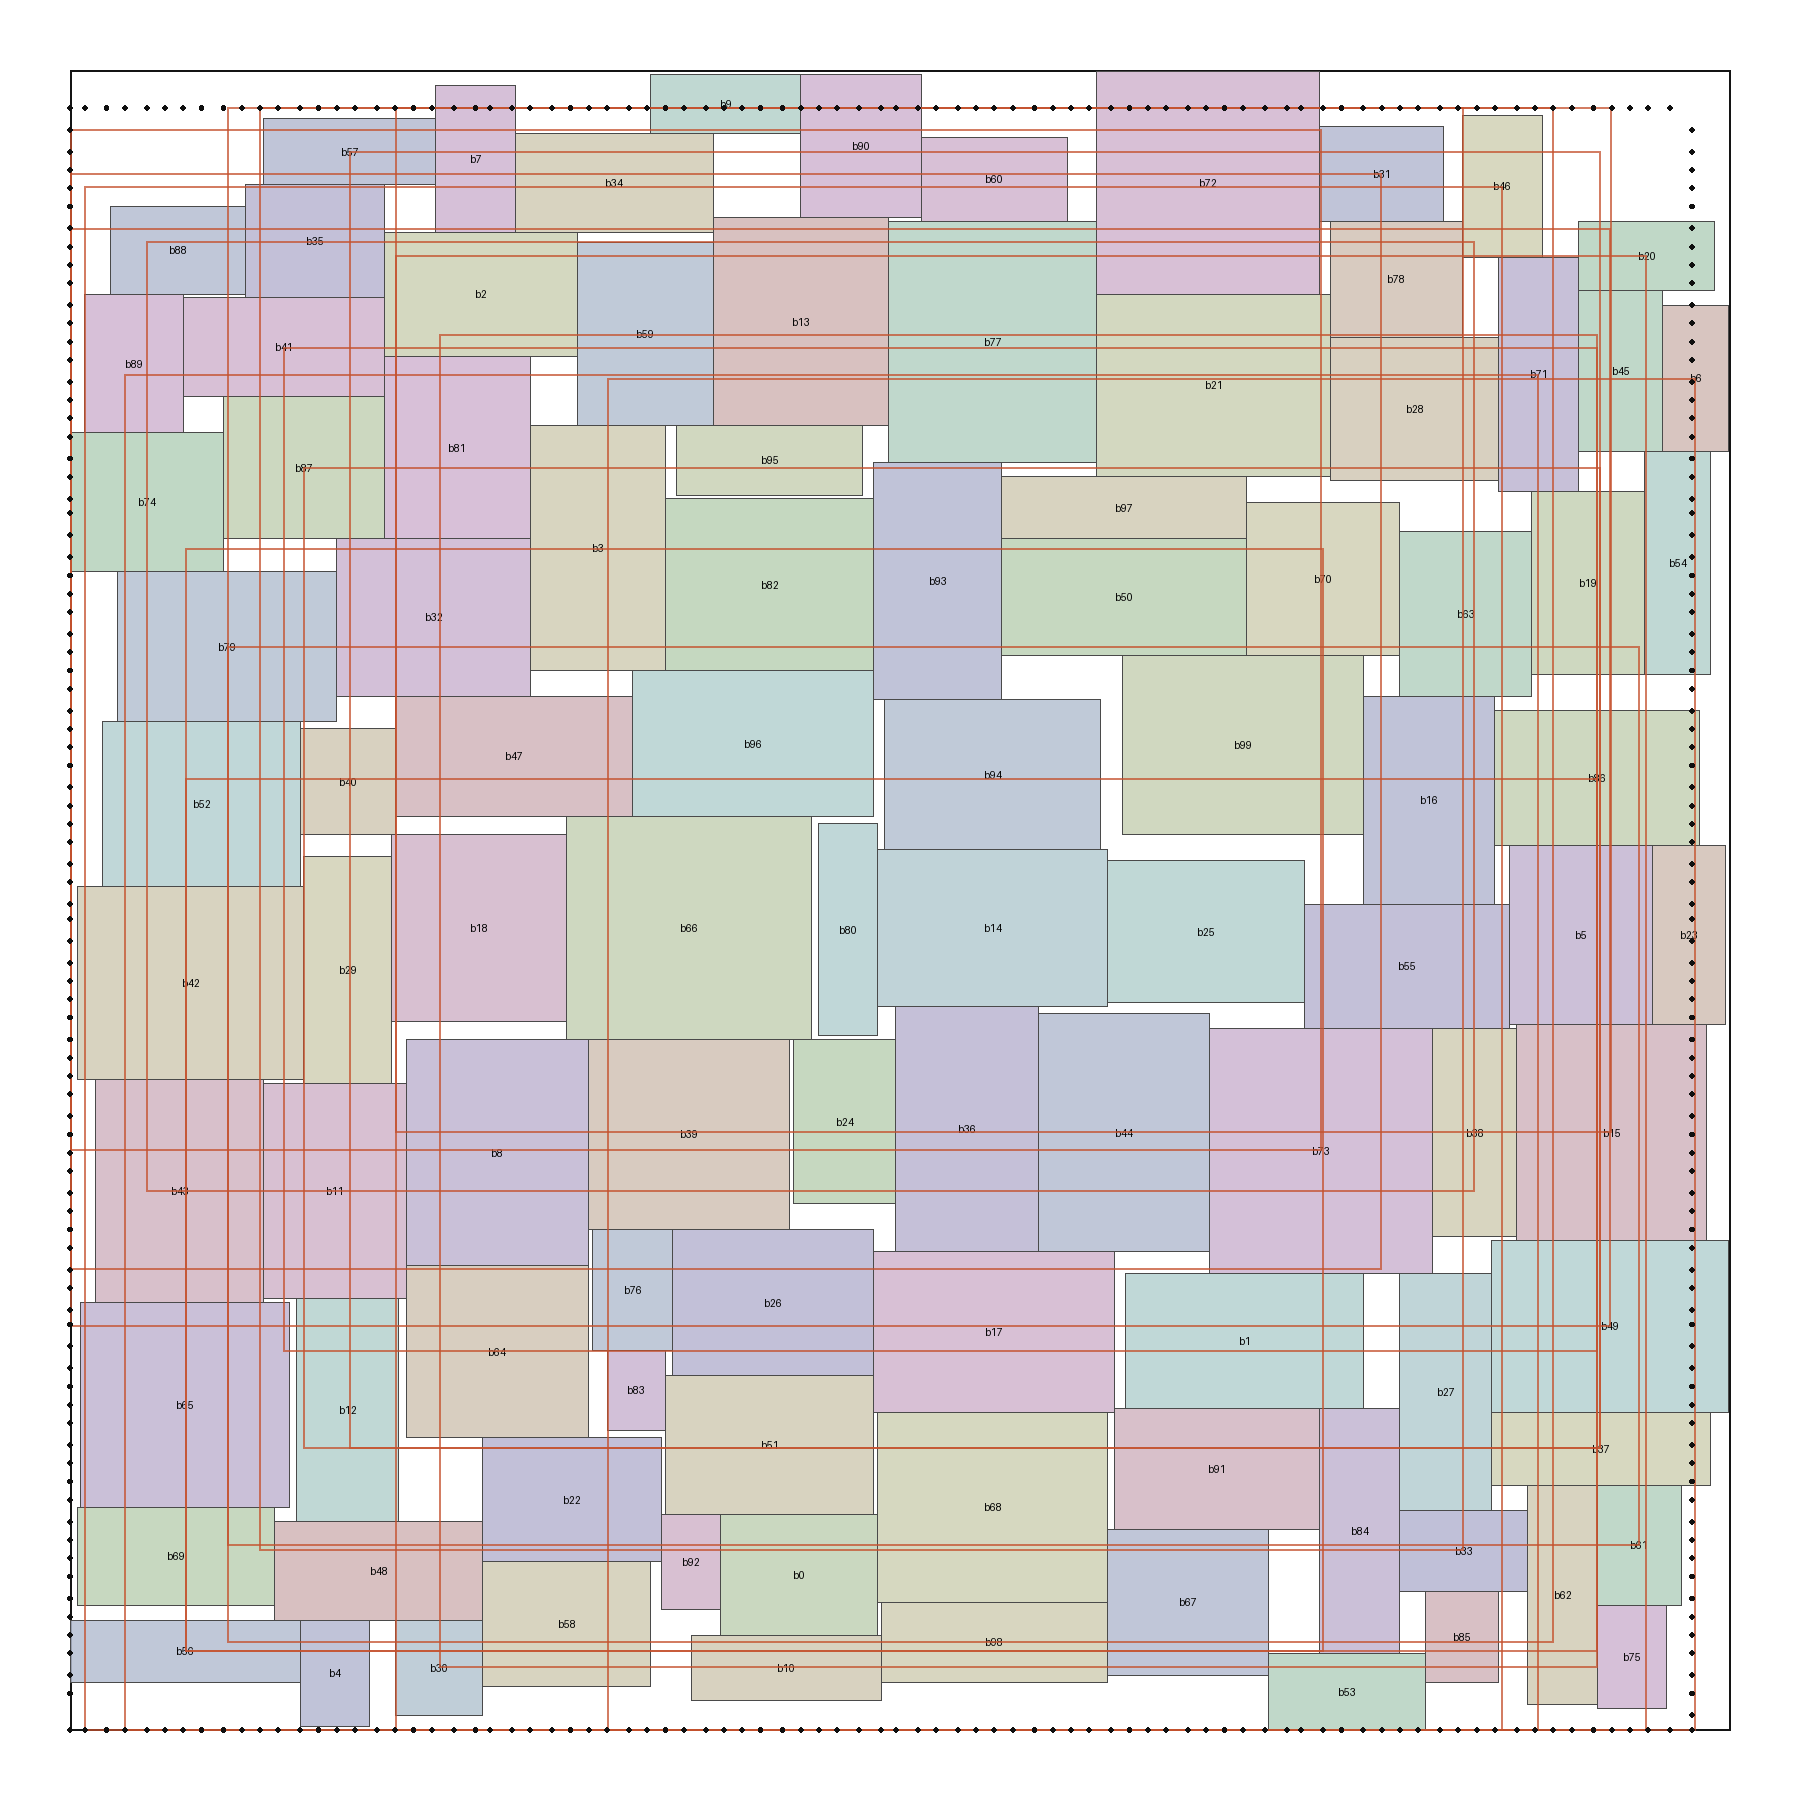
\includegraphics[width=\textwidth]{../results/q2/figures/n100_q2_layout.png}\\[-0.3em]
    {\small (a) \texttt{n100}}
  \end{minipage}
  \hfill
  \begin{minipage}[c]{0.48\textwidth}
    \centering
    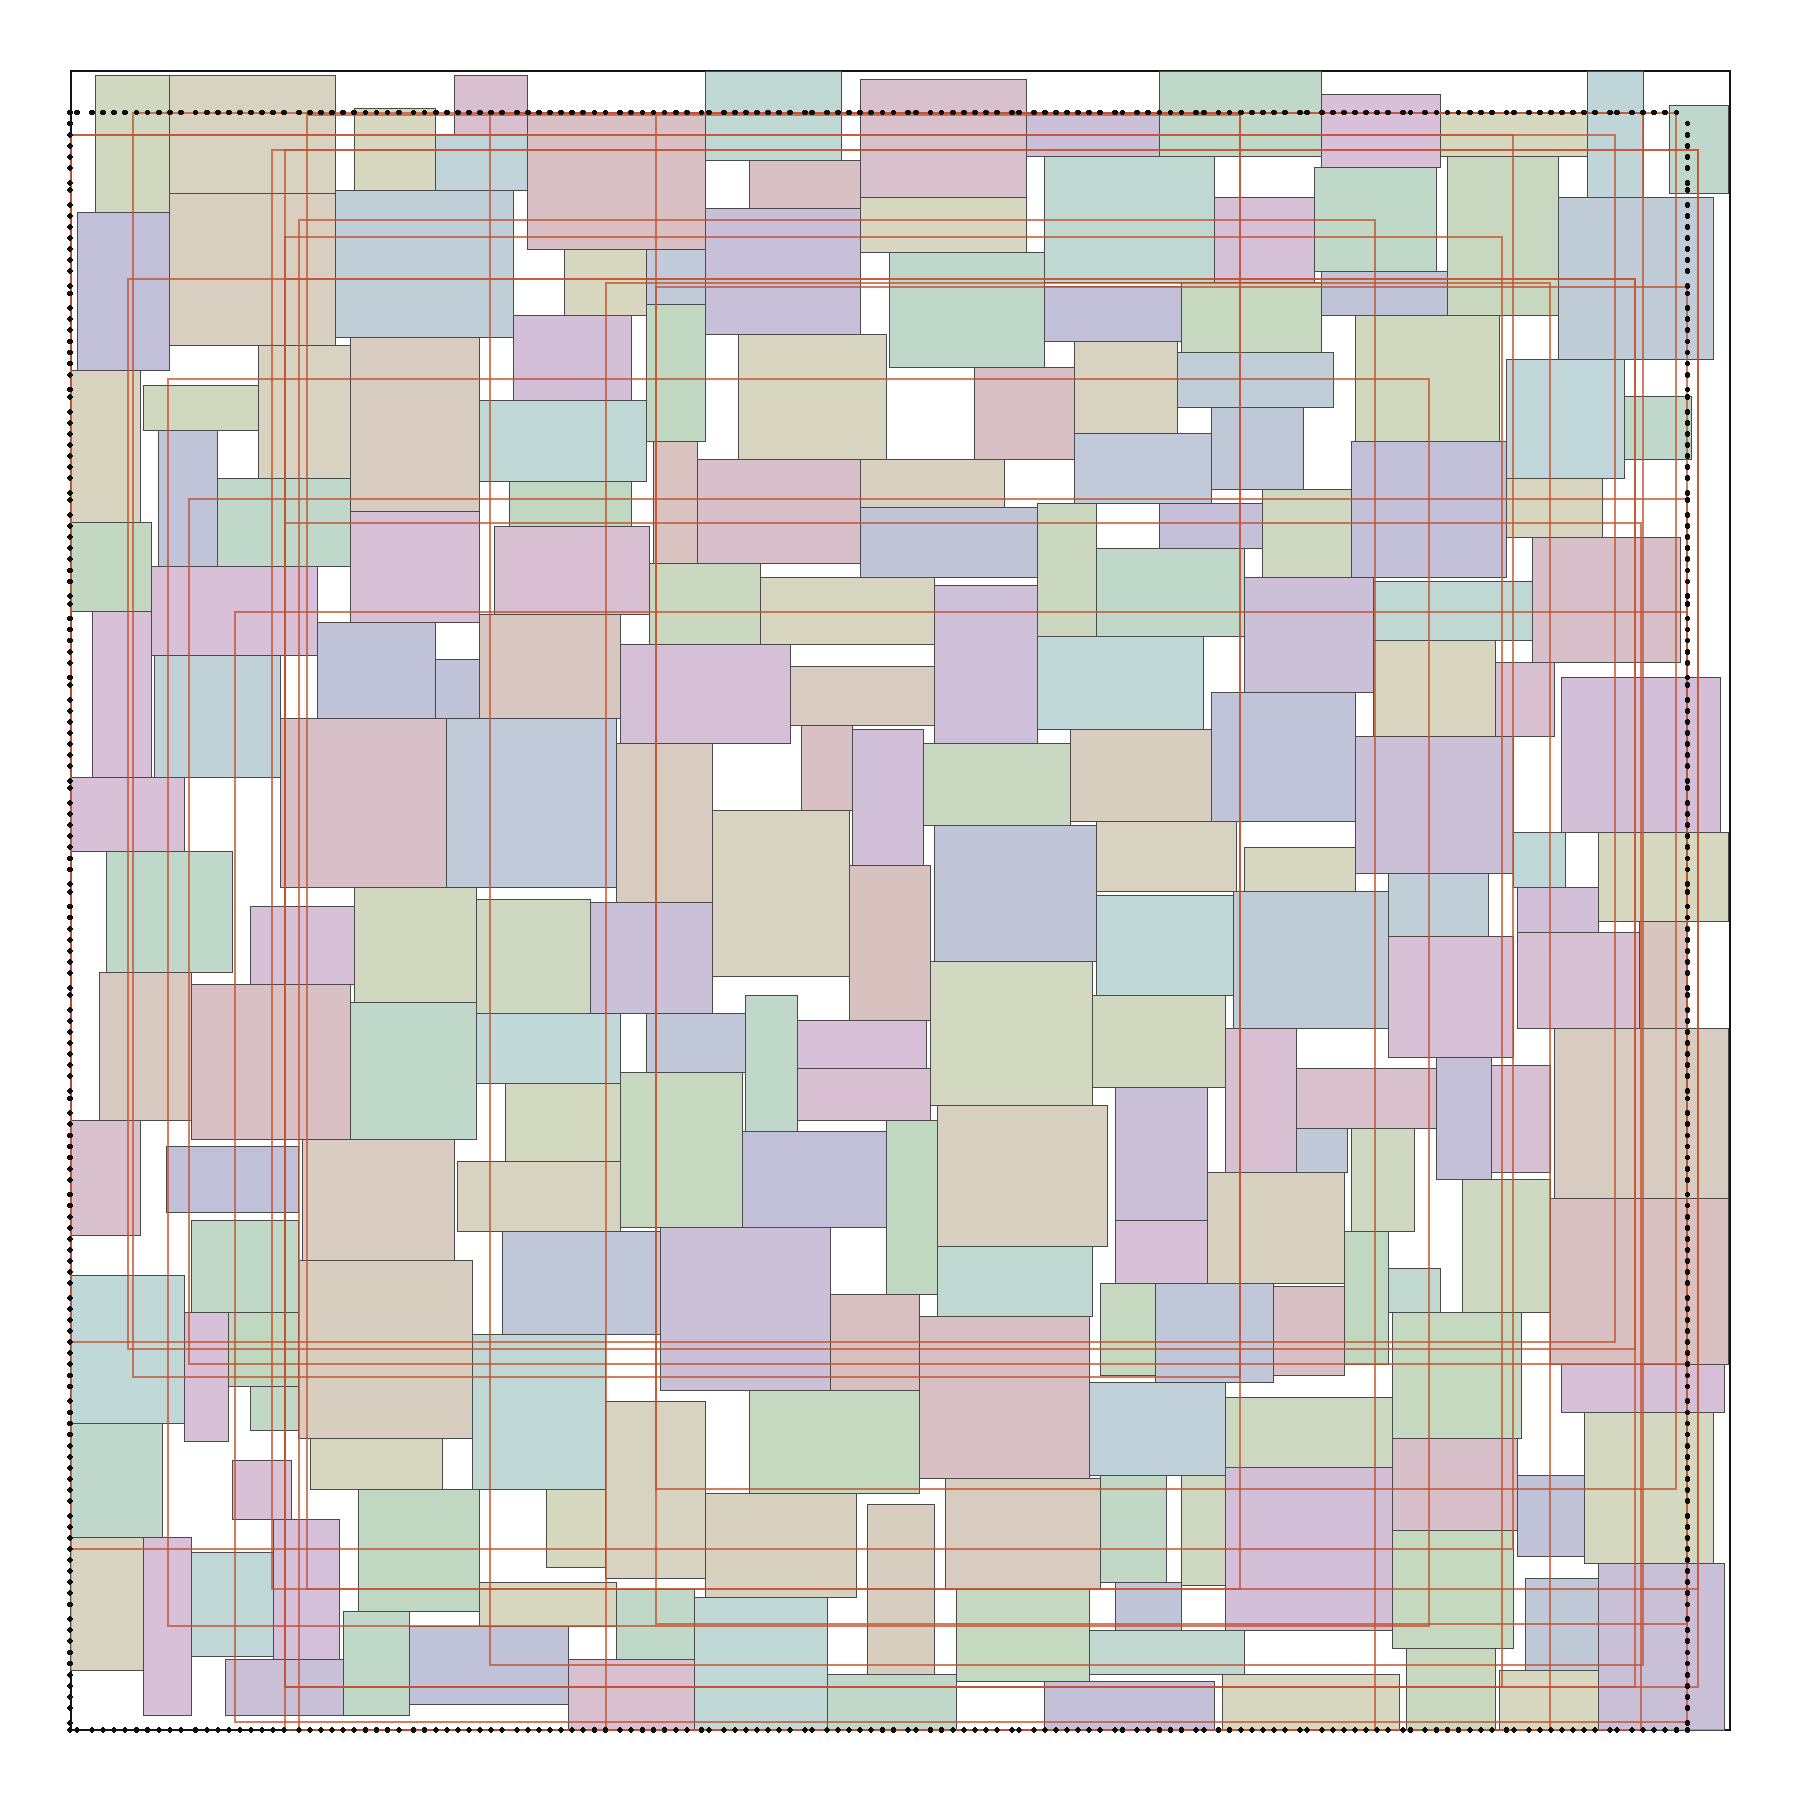
\includegraphics[width=\textwidth]{../results/q2/figures/n200_q2_layout.png}\\[-0.3em]
    {\small (b) \texttt{n200}}
  \end{minipage}
  \caption{问题二 \texttt{n100} 与 \texttt{n200} 在死区率 $0.15$ 下的固定轮廓 HPWL 布局。外黑框为连续正方形轮廓。}
  \label{fig:q2_n100_n200}
\end{figure}

两组布局均将全部模块限制在正方形边界内，同时保留由式~\eqref{eq:q2_outline}规定的空余空间。强调色网络外接框跨越多个模块区域，反映出固定 Terminal 和多引脚网络对模块相对位置的共同约束；普通模块采用低饱和配色，使视觉注意力集中于这些线长压力较高的网络。

\texttt{n300} 包含 $300$ 个硬模块和 $1893$ 条网络，其最终布局见图~\ref{fig:q2_n300}。

\begin{figure}[H]
  \centering
  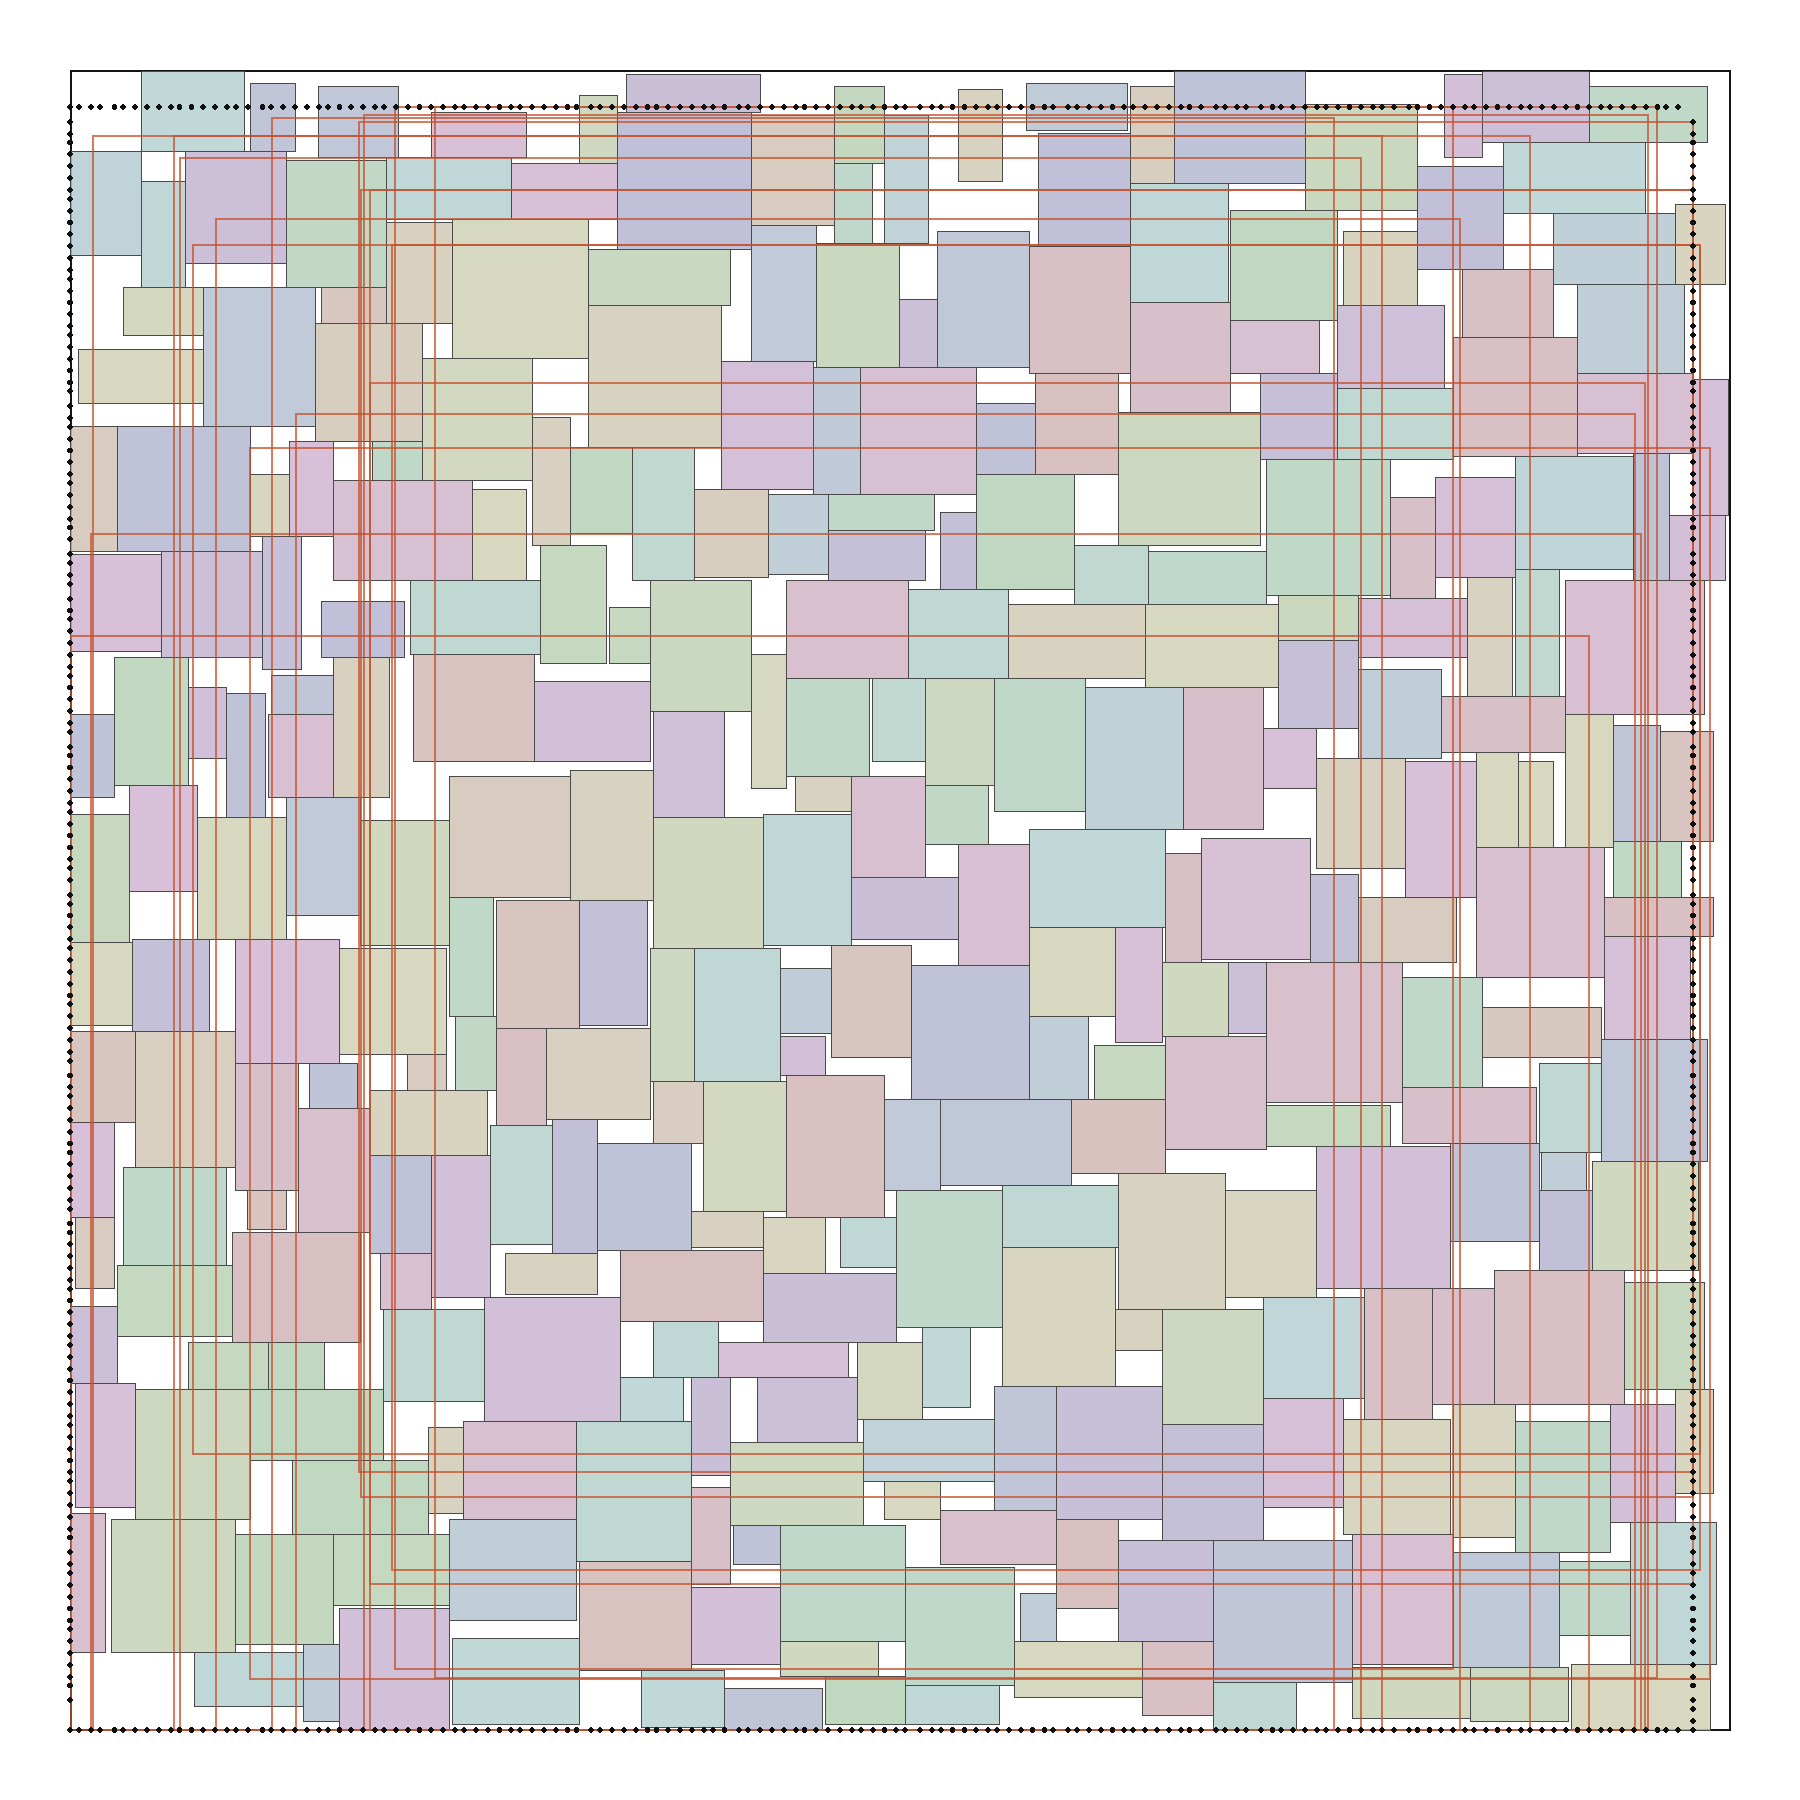
\includegraphics[width=0.88\textwidth]{../results/q2/figures/n300_q2_layout.png}
  \caption{问题二 \texttt{n300} 在连续边长 $560.487$ 的正方形轮廓内所得 HPWL 布局。白色区域为未被硬模块占用的空间。}
  \label{fig:q2_n300}
\end{figure}

在模块和网络规模增加后，布局仍满足相同的固定轮廓与死区率定义。其最终半周长线长为 $560492.5$，相较局部优化前降低 $3488.5$，说明断点局部搜索在保持几何可行性的同时进一步缩短了网络外接框半周长之和。固定轮廓矩形布局含有大规模析取约束，二次松弛、合法化和局部重插入均属于启发式求解，因此上述 HPWL 是经验证的可行结果，不构成全局最优性证明。

\subsection{模型结果检验}

三组最终布局均通过模块完整性、连续轮廓边界、两两非重叠、模块总面积一致性与 HPWL 独立复算检验；详细复核结果移至附录表~\ref{tab:appendix_q2_validation}。

问题二在死区率 $0.15$ 的固定正方形轮廓内完成三组硬模块布局，所得总\allowbreak HPWL 分别为\allowbreak $220279.0$、$410072.5$ 和 $560492.5$。结果表明，网络驱动目标中心为几何布局提供了方向，但初始合法化保留网络结构的程度仍会影响局部搜索后的最终 HPWL；本问方法可进一步用于问题三不同死区率下的布局求解。
